% Andrzej Kalinowski 2026, Wstęp do Metod Numerycznych

\documentclass[12pt,a4paper]{article}

\usepackage[utf8]{inputenc}
\usepackage[T1]{fontenc}
\usepackage[provide=*,polish]{babel}
\usepackage{lmodern}
\usepackage{amsmath, amssymb, mathtools}
\usepackage{graphicx, float, booktabs, siunitx, microtype}
\usepackage[a4paper, margin=2.5cm]{geometry}
\usepackage[hidelinks]{hyperref}
\renewcommand{\arraystretch}{1.5}
\setlength{\arraycolsep}{10pt}

\title{\textbf{Kulka spadająca na wietrze}\\[0.3em]\large Wstęp do Metod Numerycznych - Podsumowanie projektu, Zadanie 13}
\author{Andrzej Kalinowski}
\date{\today}

\begin{document}
\maketitle

% \begin{abstract}
% \noindent Krótkie streszczenie
% \end{abstract}

\section{Wprowadzenie}

Zadanie polega na obliczniach numerycznych ruchu kulki spadającej z uwzględnieniem oporu powietrza
 oraz zadanego wydatku podmuchu powietrza.
\begin{figure}[H]
    \centering
    \IfFileExists{images/zadanie-rysunek.pdf}{%
        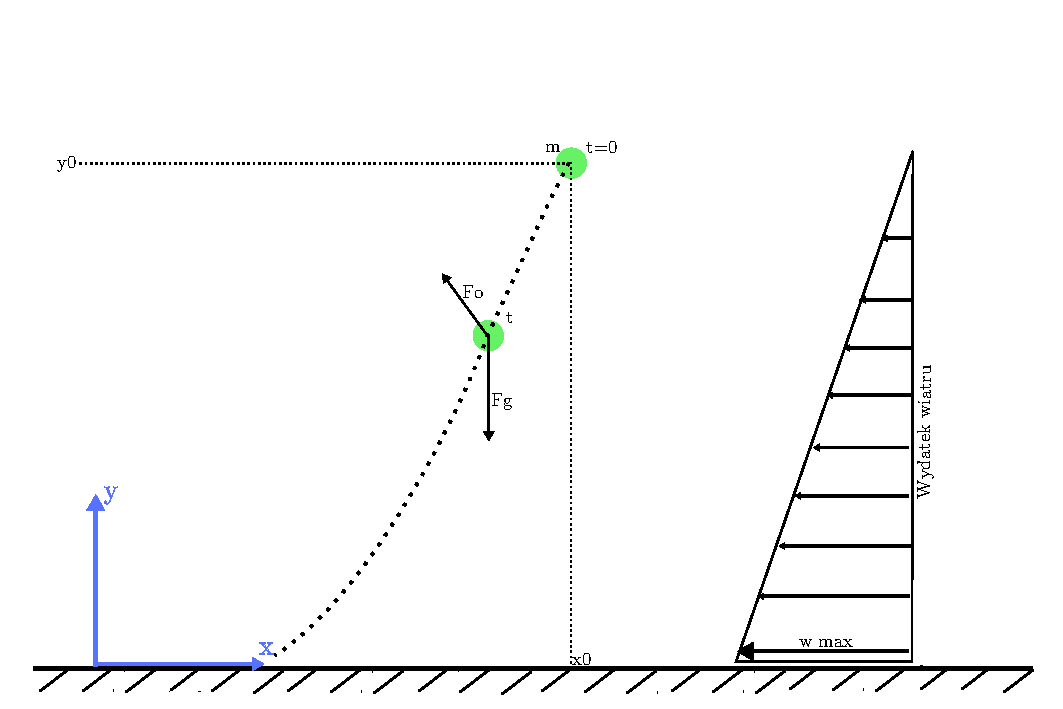
\includegraphics[width=1.1\linewidth]{images/zadanie-rysunek.pdf}%
    }{%
        \fbox{Brak pliku rysunku}%
    }
    \caption{Schemat zadania.}
    \label{fig:schemat}
\end{figure}

\section{Notacja i oznaczenia}
\begin{itemize}
    \item $m$ --- masa kulki \si{kg}
    \item $\vec{r}(t)$ --- położenie kulki w funkcji czasu \si{s}
    \item $x(t)$, $y(t)$ --- składowe położenia kulki w funkcji czasu \si{m}
    \item $y_0, x_0$ --- warunki początkowe położenia kulki \si{m}
    \item $\vec{v(t)} = \dot{\vec{r}}(t)$ --- prędkość kulki \si{m/s}
    \item $\vec{a(t)} = \ddot{\vec{r}}(t)$ --- przyspieszenie kulki \si{m/s^2}
    \item $\vec{F_w}(t)$ --- siła wypadkowa działająca na kulkę \si{N}
    \item $\vec{F_g}$ --- siła grawitacji \si{N}
    \item $\vec{F_o}$ --- siła oporu powietrza \si{N}
    \item $\vec{w}(t)$ --- wektor prędkości wiatru \si{m/s}
    \item $\vec{v_p(t)}$ --- prędkość względna kulki względem powietrza \si{m/s}
    \item $w_{max}$ --- maksymalna prędkość wiatru \si{m/s}
    \item $g$ --- przyspieszenie ziemskie \si{m/s^2}
    \item $\rho$ --- gęstość powietrza \si{kg/m^3}
    \item $S$ --- pole przekroju poprzecznego \si{m^2}
    \item $C$ --- współczynnik oporu aerodynamicznego
\end{itemize}

\section{Wyprowadzenie równań ruchu}
Równania ruchu zostały wyprowadzone przy użyciu drugiej zasady dynamiki $\vec{a} = \frac{\vec{F}}{m}$ oraz wzoru na siłę oporu powietrza $F_o = \frac{\rho v^2}{2} S C$.

\begin{equation}
    \vec{F_g}(t) = 
    \begin{bmatrix}
        0 & -mg & 0
    \end{bmatrix}
\end{equation}
Pomoczniczo wprowadzamy $k = \frac{1}{2}\rho S C$. Otrzymujemy wektor siły oporu powietrza:
\begin{equation}
    \vec{F_0}(t) = k \vec{v_p} |\vec{v_p}|
\end{equation}
\begin{equation}
    \vec{F_0}(t) = 
    \begin{bmatrix}
        k |\vec{v_p}| v_{px} & k |\vec{v_p}| v_{py} & 0
    \end{bmatrix}
\end{equation}
Siła wypadkowa:
\begin{equation}
    \vec{F_w}(t) = \vec{F_g}(t) + \vec{F_0}(t) = 
    \begin{bmatrix}
        k |\vec{v_{p}}| v_{px} & k |\vec{v_{p}}| v_{py} - mg & 0
    \end{bmatrix}
\end{equation}
Prędkość wiatru - prosta opisujaca linowa zmiane predkosci wiatru od wysokosci:
\begin{equation}
    \vec{w}(t) = 
    \begin{bmatrix}
        \dfrac{w_{max}}{y_0} y(t) - w_{max} & 0 & 0
    \end{bmatrix}
\end{equation}
Prędkość względna kulki względem powietrza:
\begin{equation}
    \vec{v_p}(t) = \vec{v}(t) + \vec{w}(t) =
    \begin{bmatrix}
        \dot{x}(t) + \left( \dfrac{w_{max}}{y_0} y(t) - w_{max} \right) & \dot{y}(t) & 0
    \end{bmatrix}
\end{equation}
\begin{equation}
    |\vec{v_p}(t)| = \sqrt{\left( \dot{x}(t) + \dfrac{w_{max}}{y_0} y(t) - w_{max} \right)^2 + \dot{y}(t)^2}
\end{equation}
Przyspieszenie kulki:
\begin{equation}
    \vec{a}(t)  = 
    \begin{bmatrix}
        \ddot{x}(t)  & \ddot{y}(t)  & 0
    \end{bmatrix}
    \label{eq:acc_vector}
\end{equation}

\begin{equation}
    \vec{a}(t) = \frac{\vec{F_w}(t)}{m} =
    \begin{bmatrix}
        \dfrac{k |\vec{v_{p}}| v_{px}}{m}  & \dfrac{k|\vec{v_{p}}| v_{py} - mg}{m}  & 0
    \end{bmatrix}
    \label{eq:acc_force}
\end{equation}
Zatem, z równań~\eqref{eq:acc_vector} i~\eqref{eq:acc_force} otrzymujemy układ równań różniczkowych:
\begin{equation}
    \begin{cases}
        \ddot{x}(t) = \dfrac{k |\vec{v_{p}}| v_{px}}{m}, \\
        \ddot{y}(t) = \dfrac{k|\vec{v_{p}}| v_{py} - mg}{m}.
    \end{cases}
\end{equation}
Po podstawieniu opdowiednich zależności, otrzymujemy ostateczny układ równań różniczkowych:
\begin{equation}
    \begin{cases}
        \ddot{x}(t) = \dfrac{k |\vec{v_{p}}| (\dot{x}(t) + \dfrac{w_{max}}{y_0} y(t) - w_{max})}{m}, \\
        \ddot{y}(t) = \dfrac{k|\vec{v_{p}}| \dot{y}(t) - mg}{m}.
    \end{cases}
\end{equation}

\section{Metoda rozwiązania}
Do rozwiązania układu użyto metody Rungego-Kutty 4 rzędu (RK4), zaimplemenmtowany w C.
Aby takie rozwiązanie było możliwe układ sprowadzono do postaci układu równań różniczkowych pierwszego rzędu.
\begin{equation}
    \begin{cases}
        z_1 = x(t) \\
        z_2 = \dot{x}(t) \\
        z_3 = y(t) \\
        z_4 = \dot{y}(t) \\
    \end{cases}
\end{equation}
\begin{equation}
    \begin{cases}
        \dot{z_1} = z_2 \\
        \dot{z_2} = \dfrac{k |\vec{v_{p}}| (z_2 + \dfrac{w_{max}}{y_0} z_3 - w_{max})}{m} \\
        \dot{z_3} = z_4 \\
        \dot{z_4} = \dfrac{k|\vec{v_{p}}| z_4 - mg}{m} \\
    \end{cases}
\end{equation}
Taki układ można rozwiązań wktororową metodą RK4.

\section{Parametry obliczeń}
Do wykonania obliczeń użyto następujących parametrów:
\begin{table}[H]
    \centering
    \begin{tabular}{@{}lcl@{}}
        \toprule
        \textbf{Parametr} & \textbf{Symbol} & \textbf{Wartość} \\
        \midrule
        Masa      & $m$ & \SI{0.1}{kg}    \\
        Promień kulki & $R$ & \SI{0.1}{m}     \\
        Maksymalna prędkość wiatru & $w_{max}$ & \SI{25}{m/s} \\
        Wysokosc poczatkowa & $y_0$ & \SI{10}{m} \\
        Położenie początkowe w osi x & $x_0$ & \SI{10}{m} \\    
        Prędkość początkowa w osi x & $vx_0$ & \SI{0}{m/s} \\
        Prędkość początkowa w osi y & $vy_0$ & \SI{0}{m/s} \\
        Przyspieszenie ziemskie & $g$ & \SI{9.81}{m/s^2} \\
        Gęstość powietrza & $\rho$ & \SI{1.225}{kg/m^3} \\
        Współczynnik oporu & $C$ & 0.3 \\
        Krok całkowania     & $dt$ & \SI{0.001}{s}    \\
        \bottomrule
    \end{tabular}
    \caption{Parametry użyte w symulacji.}
    \label{tab:params}
\end{table}

\section{Wyniki}
Wynki obliczeń zostały przeadstawione na wykresach, które zostały wygenerowane przy użyciu skryptu w Pythonie.
Przy zadanych parametrach kulka spadnie na ziemię po około \underline{\SI{1.176}{s}.}

\begin{figure}[H]
    \centering
    \includegraphics[width=1.1\linewidth]{plots/Trajektoria kulki.pdf}
    \caption{Tor ruchu kulki.}
    \label{fig:polozenie}
\end{figure}

\begin{figure}[H]
    \centering
    \includegraphics[width=1\linewidth]{plots/Położenie kulki w osi x.pdf}
    \caption{Położenie kulki w osi x.}
    \label{fig:położenie_x}
\end{figure}

\begin{figure}[H]
    \centering
    \includegraphics[width=1\linewidth]{plots/Położenie kulki w osi y.pdf}
    \caption{Położenie kulki w osi y.}
    \label{fig:położenie_y}
\end{figure}
\begin{figure}[H]
    \centering
    \includegraphics[width=1\linewidth]{plots/Prędkość kulki w osi x.pdf}
    \caption{Prędkość kulki w osi x.}
    \label{fig:predkosc_x}
\end{figure}
\begin{figure}[H]
    \centering
    \includegraphics[width=1\linewidth]{plots/Prędkość kulki w osi y.pdf}
    \caption{Prędkość kulki w osi y.}
    \label{fig:predkosc_y}
\end{figure}
\begin{figure}[H]
    \centering
    \includegraphics[width=1\linewidth]{plots/Energia mechaniczna kulki.pdf}
    \caption{Całkowita energia mechaniczna kulki.}
    \label{fig:energia}
\end{figure}

\section{Wnioski}

Projekt polegasł na rozwiązaniu układu mechanicznego reprezenotowanego przez zestaaw rówanń różniczkowych.
Równania zostały wyprowadzone przy użyciu drugiej zasady dynamiki oraz wzoru na siłę oporu powietrza
oraz rozwiązane numerycznie przy użyciu metody Rungego-Kutty 4 rzędu.
Uzyskane wyniki są zgodne z oczekiwaniami - kula spada.

Ciekawą obserwacją jest fakt że podmuch wiatru, mimo że działa wyłącznie poziomo to wpływa równiwez na ruch w osi pionowej.

\end{document}
